\chapter{Acquaintance and first steps }
This chapter is devoted to a first acquaintance with possibilities which Mathapar opens.
The language MathPar, which is described below, may be considered as a kind of development of a TeX language.
TeX serves for writing mathematical texts and preparing them for publication. It may be called "passive" 
in comparison with the language MathPar, which permits to execute computations, and so is a self-depended mathematical language. A problem definition and a result of computations are written in MathPar.

Just after computations you see the whole mathematical text  as a pdf-image which is accustomed 
in scientific and technical publications.

The result may be further used in different ways.

(1) You may click the text with your mouse, and it would return to the initial form of the MathPar language. 
Then you may continue to edit the text or pass to a next task. There is another way to change a form  of a text~--- 
using a button%begindelete 
\ <<
\includegraphics[scale=0.6]{pictures/button_arrows.png}>>%enddelete
, placed between buttons <<$\blacktriangleright$>> and <<$+$>>.
 

(2) You may click {\bf the image of the mathematical text} with the right mouse button, and the drop-down menu appears. The upper field {\bf Show-Math-As} permits to pass to the choice of language. 
It is suggested to chose  
Tex or MathML. You may open a field you need.

For example, a matrix of the size $2\times 2$ will be written in MathPar in the following way:

A=[[a,b],[c,d]];

in TeX as follows:

A= $\backslash$left(\comm{begin}{\{array\}}\{${cc}$\}$ a \& b$ $\backslash\backslash c \& d \backslash\backslash$ \comm{end}{\{array\}}$\backslash$right).

In MathML it is much more complicated.

The text obtained in Tex or in MathML you may copy and past into TeX or HTML file and use for publication. You may also save it as an image and use in any document. It is useful, for example, when it is necessary to save a plot or a solution of a problem 


\section{Input data and run the calculations}

At the center of the screen there is an entry field where it is possible to enter
 mathematical expressions.
 To start a task press the button $\blacktriangleright$.  When your cursor is disposed in the field of input you can press the combination  of keys {\it Ctrl+Enter}.


%begindelete
Example  is shown in figure 2.1.  
 
\begin{figure}
  \label{1_1}
  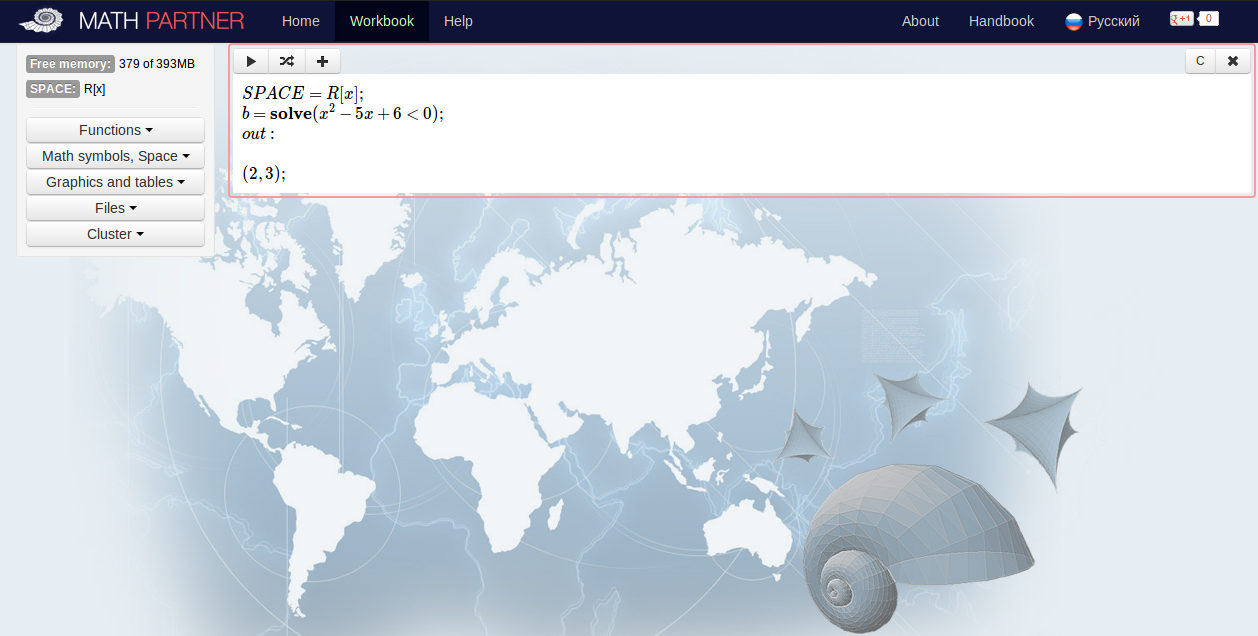
\includegraphics[scale=0.5]{pictures/1_1e}
  \caption{Entering data into a working page}
\end{figure}
%enddelete

On the top of the screen you can see buttons ${\small \fbox {Help}}$ and ${\small \fbox{Handbook}}$. 
This is way to the help files. All the fields of the help pages are active, and you can run the help examples. You can copy text from the samples and transfer them into the field for user input.

When you enter mathematical expressions, they must be separated by a semicolon (;) or text comments, which are enclosed in quotation marks.
 
When you need to have a mathematical expression in the comment as part of the comment, it must be skirted in the dollar signs ($\$$). For example, you can write a comment:

\noindent
$"$ Two different notations $\$ \backslash exp(x)\$$ and $\$\backslash e  \widehat{\ }{} x\$$  are used for the exponential function.$"$

To obtain results it is necessary to use the command \comm{print}{()} and to specify the names of those
 expressions which are required to be printed. 

If the list of statement does not contain a print statement \comm{print}{()} or any other operator (\comm{plot}{()}, \comm{prints}{()}, etc.),  it will be shown the result obtained in the last statement.
  
All commands or operators should begin with the symbol <<back slash>> ($\backslash$).  
 
 
The button $\fbox{+}$ lets us add new entry fields. You can press the combination of
 keys {\it Crtl+Del} to remove this field or you can press the button $\fbox{x}$ at the right side of this field on the screen.
 
The button $\fbox{C}$ is designed to clean the values of all previously typed names. 
It is useful to have such button when the numerical values are entered in some sections, and the calculations are done in other sections. 
Clearing all names allows you to obtain a symbolic expression rather than the number.

On the left of the screen you can see fields with a current environment and a current random access memory. Under the fields differant buttons for enter of functions are placed.


\subsection{Working with files}
Functions for working with files are available at the "Files" collapsible panel from menu at the left.

Here is what you can do with files:

1) Save the result of the last run section as PDF file with "Save PDF" button. You can specify desirable
paper size (dimensions are in centimeters), by default page has size A4 (21x29.7 cm)

2) Upload text files to Mathpar server with "Upload file" button. 
Under the button there is a list of uploaded files. 
Files should contain Mathpar expressions or tables in specific format.

Table contains of header -- it's the first row with arbitrary strings in it -- and
number rows. Columns are separated with tabulation symbol. Functions for working 
with tables are available at the panel "Graphics and tables" (see also 
section 3.1 Plotting functions of help system).

3) Input Mathpar expressions from uploaded files with \comm{fromFile}{()} function.
E.g., to make an expression from file myfile.txt and assign this expression to 
variable $a$ run: a = \comm{fromFile}{('myfile.txt')}.

\section{Mathematical functions}
The following notations for elementary functions and constants are accepted.
\subsection{Constants}  
\hspace*{4mm}  $\backslash$i~--- imaginary unit, 

 $\backslash$e~--- the basis of natural logarithm,  

 $\backslash$pi~--- the ratio of length of a circle to its diameter,    

 $\backslash$infty~--- infinity sign. 


\subsection{Functions of one argument} 

\hspace*{4mm} $\backslash$ln --- natural logarithm, 

 $\backslash$lg --- decimal logarithm, 

 $\backslash$sin --- sine,  

 $\backslash$cos --- cosine,  

 $\backslash$tg --- tangent,  

 $\backslash$ctg --- cotangent, 

 $\backslash$arcsin --- arcsine, 

 $\backslash$arccos --- arccosine,  

 $\backslash$arctg --- arctangent,  

 $\backslash$arcctg --- arccotangent, 

 $\backslash$sh --- sine hyperbolic, 

 $\backslash$ch --- cosine hyperbolic, 

 $\backslash$th --- tangent hyperbolic, 

 $\backslash$cth --- cotangent hyperbolic, 

 $\backslash$arcsh --- arcsine hyperbolic, 

 $\backslash$arcch --- arccosine hyperbolic,  

 $\backslash$arcth --- arctangent hyperbolic, 

 $\backslash$arccth --- arccotangent hyperbolic, 

 $\backslash$exp --- exponent,  

 $\backslash$sqrt --- root square, 

 $\backslash$abs --- absolute value of real numbers (module for complex numbers),

 $\backslash$sign --- number sign (returns $1$, $0$, $-1$ when number sign is $+$, $0$, $-$, correspondingly),
 
 $\backslash$unitStep$(x,a)$ --- is a function which, for $ x> a $ takes the value $ 1 $, and
for $ x <a $ takes the value $ 0 $;

 $\backslash$fact --- factorial.  It is defined for positive integers. It is equivalent to  $n!$.

\subsection{Functions of two arguments} 
\hspace*{4mm}  $\widehat{\ }{}$ --- degree, 

 $\backslash$log --- logarithm of function with given base, 

 $\backslash$rootOf(x, n) --- root of degree n of x, 

 $\backslash$Gamma --- the function Gamma, 

 $\backslash$Gamma2 --- the function Gamma 2,  

 $\backslash$binomial --- binomial coefficient. 


\smallskip

\underline{Example.}

\vspace*{-3mm}
\begin{verbatim}
SPACE = R64[x, y];
f1 = \sin(x);
f2 = \sin(\cos(x + \tg(y)));
f3 = \sin(x^2) + y;
\print(f1, f2, f3);
\end{verbatim}\vspace*{-3mm}
%begindelete

Returns:\\
$SPACE=R64[x,y];$\\
$f1 = sin(x);$\\
$f2 = sin(cos(x+tg(y)));$\\
$f3 = sin(x^{2})+y.$
%enddelete

\section{Actions with functions}

For the above functions and their compositions, you can calculate the value of the function at the point,   substitute the expression into a function instead of arguments, calculate the limit of the function,  calculate derivative, etc. For this purpose, the following commands are defined.



To calculate the value of a function at a point you must run 
\comm{value}{(f, [var1, var2, \ldots, varn])},
where $f$~---function, and 
$var1, var2, \ldots, varn $~--- values 
of the variables of the 
ring.

 For the substitution of expressions to the function you must execute the 
\comm{value}{(f, [func1, func2, \ldots, funcn])}, where $ f $~--- a function
$ func1, func2, \ldots, funcn $~--- expressions that are substituted for the corresponding variables.

 To calculate the limit of a function at a point you must run 
\comm{lim}{(f, var)},
where $ f $~--- this function, and $ var $~--- the point at which you want to find the limit.

 In order to calculate the derivative of 
$f$ in the variable 
$y$ in the ring $\mathbb {Z} [x, \ y, \ z]$
  you must run \comm{D}{(f, y)}. To find a mixed first-order derivative of the function $ f $ there is a command
\comm{D}{(f, [x, y])}, to find the derivative of higher order you must use the command  $\backslash {\mathbf {D}} (f, [x \widehat{\ }{} k, z \widehat{\ }{} m, y \widehat{\ }{} n])$, 
where $ k, m, n $ indicate the order of the derivative of variables.




\smallskip

\underline{Examples. }

\vspace*{-2mm}
\begin{verbatim}
SPACE = R[x, y];
f = \sin(x^2 + \tg(y^3 + x));
g = \value(f, [1, 2]);
\print(g);
\end{verbatim}\vspace*{-2mm}
%begindelete

Returns:\\
in: $SPACE=R[x, y];$\\ 
\hspace*{4mm} $f=sin(x^2+tg(y^3+x)); $\\
\hspace*{4mm} $g=value(f,\ [1,\ 2]); $\\
\hspace*{4mm} $print(g);$\\
out: $g = 0. 52;$\\

%enddelete
\vspace*{-2mm}
\begin{verbatim}
SPACE = Z[x, y];
f = x + y;
g = f^2;
r = \value(f, [x^2, y^2]);
\print(g, f, r);
\end{verbatim}\vspace*{-2mm}
%begindelete

Returns: \\
in: $SPACE=Z[x, y]; $\\
\hspace*{4mm} $f=x+y;$\\ 
\hspace*{4mm} $g=f^2; $\\
\hspace*{4mm} $r=value(f, [x^2, y^2]); $\\
\hspace*{4mm} $print(g, f, r);$\\
out: $g = y^{2}+2yx+x^{2}; $ \\
\hspace*{4mm} $f = y+x;$ \\ 
\hspace*{4mm} $r=x^2+y^2 $

%enddelete
\vspace*{-3mm}
\begin{verbatim}
SPACE = R64[x];
f = \sin(x) / x;
g = \lim(f, 0);
\print(g);
\end{verbatim}\vspace*{-3mm}
%begindelete

Returns: \\
in: $ SPACE=R64[x]; $\\
\hspace*{4mm} $f=sin(x)/x; $\\
\hspace*{4mm} $g=lim(f, 0); $\\
\hspace*{4mm} $print(g);$\\
out: $g = 1. 00;$

%enddelete
\vspace*{-3mm}
\begin{verbatim}
SPACE = Z[x, y];
f = \sin(x^2 + \tg(y^3 + x));
h = \D(f, y);
\print(h);
\end{verbatim}\vspace*{-3mm}
%begindelete

Returns:\\
in: $SPACE=Z[x, y]; $\\
\hspace*{4mm} $f=sin(x^2+ tg(y^3+x)); $\\
\hspace*{4mm} $h= D(f, y);$\\ 
\hspace*{4mm} $print(h);$\\
out: $h = 3y^2 cos(x^2+tg(y^3+x))/(cos(y^3+x))^2;$
%enddelete

\section{Solution of the algebraic equation}  
 
To obtain a solution of the algebraic equation use the command  \comm{solve}{}.

 The command <<FLOATPOS = N>> is used for setting the environment. It sets the number of decimal places after the decimal point $ (N) $, which should appear in the print of the numerical results of approximate calculations. It is not connected with the process of calculation, but only with printing. By default, $ FLOATPOS = 2 $.

\underline{Examples. }

\vspace*{-2mm}
\begin{verbatim}
SPACE = R64[x];
b = \solve(x^2 - 5x + 6 = 0);
\end{verbatim}
%begindelete

\ex{$SPACE=R64[x]; $\\
\hspace*{4mm} $b=solve(x^2-5x+6=0);$ }{$[2. 00, 3. 00];$}

%enddelete
\begin{verbatim}
SPACE = R64[x];
FLOATPOS = 6;
b = \solve(x^4 + 2x + 1 = 0);
\end{verbatim}
%begindelete

\ex{$SPACE=R64[x];$\\ 
\hspace*{4mm} $FLOATPOS=6; $\\
\hspace*{4mm} $b=solve(x^4 +2x +1=0);$}{$[-0.543689,-1.000000];$} 

%enddelete
\begin{verbatim}
SPACE = R64[x];
FLOATPOS = 0;
b = \solve(x^3 + 3x^2 + 3x + 1 = 0);
\end{verbatim}
%begindelete

\ex{$SPACE=R64[x]; $\\
\hspace*{4mm} $FLOATPOS=0;$\\
\hspace*{4mm} $b=solve(x^3+3x^2+3x+1=0);$}{$-1$.}
%enddelete

\section{Solution of the algebraic inequalities}

To obtain a solution of the algebraic inequalities use the command  \comm{solve}{}, which contains the inequalities.
We can solve strict and not strict algebraic inequalities. Open interval is indicated in parentheses ( ), closed interval is indicated inbrackets [ ], set is denoted by braces \{ \}.

\underline{Examples. }

\begin{verbatim}
SPACE = R[x];
b = \solve(x^2-5x+6 < 0);
\end{verbatim}
%begindelete

\ex{$SPACE=R[x]; $\\
\hspace*{4mm} $b=solve(x^2-5x+6 < 0);$}{$(2,3)$.}
%enddelete

\begin{verbatim}
SPACE = R[x];
b = \solve((x+1)^2(x-3)(x+5) \ge 0);
\end{verbatim}
%begindelete

\ex{$SPACE=R[x]; $\\
\hspace*{4mm} $b=solve((x+1)^2(x-3)(x+5) \ge 0);$}{$(-\infty,-5] \cup\{-1\}\cup[3,\infty)$.}
%enddelete

\begin{verbatim}
SPACE = R[x];
b = \solve((x^2+11x+28)/(x+5) \le 0);
\end{verbatim}
%begindelete

\ex{$SPACE=R[x]; $\\
\hspace*{4mm} $b=solve((x^2+11x+28)/(x+5) \le 0);$}{$(-\infty,-7]\cup(-5,-4]$.}
%enddelete

\begin{verbatim}
SPACE = Q[x];
b = \solve(x^2 + 4x - 7 = 0);
\end{verbatim}
%begindelete

\ex{$SPACE=Q[x]; $\\
\hspace*{4mm} $b=solve((x^2 + 4x - 7 = 0);$}{$[(\sqrt{11}+(2)),(2-\sqrt{11})];$.}
%enddelete
\section{Solution of the algebraic inequalities systems}

To obtain a solution of the algebraic inequalities systems use the command \comm{solve}{[In1, In2, ..., Ink]}, where $[In1, In2, ..., Ink]$~--- vector, where contain inequalities.
System contain strict and not strict algebraic inequalities. Open interval is indicated in parentheses (), closed interval is indicated inbrackets, set is denoted by braces \{ \}.

\underline{Examples. }

\vspace*{-2mm}
\begin{verbatim}
SPACE = R[x];
b = \solve([x^2+4x-5 > 0, x^2-2x-8 < 0]);
\end{verbatim}
%begindelete

\ex{$SPACE=R[x]; $\\
\hspace*{4mm} $b=solve([x^2+4x-5 > 0, x^2-2x-8 < 0]);$}{$(1,4)$.}
%enddelete

\begin{verbatim}
SPACE = R[x];
b = \solve([x^2-x-6 \ge 0, x^2-4x-12 < 0]);
\end{verbatim}
%begindelete

\ex{$SPACE=R[x]; $\\
\hspace*{4mm} $b=solve([x^2-x-6 \ge 0, x^2-4x-12 < 0]);$}{$(-4,-2]\cup[3,4)$.}
%enddelete

\begin{verbatim}
SPACE = R[x];
b = \solve([x^2-4 < 0, x+1 > 0, 0.5-x > 0]);
\end{verbatim}
%begindelete

\ex{$SPACE=R[x]; $\\
\hspace*{4mm} $b=solve([x^2-4 < 0, x+1 > 0, 0.5-x > 0]);$}{$(-1,0.5)$.}
%enddelete

\section{Operations on subsets of the real numbers}

To specify a subset use the command \comm{set}{((a,b),(c,d])}, where $a,b,c,d$ are numbers.
Subset may consist of open intervals indicated by parentheses ( ), half-open intervals indicated by [ ) or ( ],
segments indicated by brackets [ ] and points indicated by braces { }, or like segments.

Simple subset is denoted by the same brackets, but you need to add a backslash ($ \backslash $) in front of each bracket. 
For example $ \backslash (3,4.5) \backslash] $, $ \backslash[7, 7 \backslash]$ or $\backslash{8 \backslash}$.
The operator $ \backslash {\mathbf {set}} $ is not required.

\begin{verbatim}
SPACE = R64[x];
a = \set((-2,1),[2,5),(5.75,6],[8,8]);
\end{verbatim}
%begindelete

\ex{$SPACE=R[x]; $\\
\hspace*{4mm} $a = set((-2,1),[2,5),(5.75,6],{8});$}{$((-2.00),1.00)\cup[2.00,5.00)\cup(5.75,6.00]\cup\{8.00\}$.}
%enddelete
 

With subsets we can make the following operations: union, intersection, subtraction, calculation of 
the symmetric difference and complement set, using the commands $\backslash cup$, 
$\backslash cap$, $\backslash setminus$, $\backslash triangle$ and symbol  (') apostrophe.

 
 
\begin{verbatim}
SPACE = R64[x];
A=\(1,3\)\cup\[5,16\);
B=\(2,4\)\cup\[10,20\);
C=A\cup B;
D=A\cap B;
E=A\triangle B;
F=A \setminus B;
G=A';
\print(C,D,E,F,G);
\end{verbatim}
%begindelete

\ex{ $SPACE=R64[x]; $\\
$ A=(1,3)\cup[5,16);$\\
$B=(2,4)\cup[10,20);$\\
$C=A\cup B;$\\
$D=A\cap B;$\\
$E=A\triangle B;$\\
$F=A \setminus B;$\\
$G=A';$\\
$print(C,D,E,F,G);$}
{$C = (1,4)\cup[5,20)$\\
 $D = (2,3)\cup[10,16)$\\
 $E = (1,2]\cup[3,4)\cup[5,10)\cup[16,20)$\\
 $F = (1,2]\cup[5,10)$\\
 $G = (-\infty,1]\cup[3,5)\cup[16,\infty)$}
%enddelete


\newpage
\section{Vectors and matrices}
To define the row-vector you have to list its elements in square brackets. 

To define the matrix you must take in square brackets a list of row vectors, for example, $ A = [[1, 2], [3, 4]] $.

Element of the matrix may be obtained by specifying the row and column number in the two lower indexes of the matrix,
and an element of the vector may be obtained by specifying its number in the lower index of the vector.
The is an example for obtaining elements. You have to set $a=\backslash elementOf(A)$, and then obtain $a$\_\{$i, j$\}.  If $B$ is a vector, then you have to set $b=\backslash elementOf(B)$, and then obtain element $b$\_\{$i$\}.  
 
You can get a row of the matrix as a vector-row and column of the matrix as a column vector. The row vector obtained by specifying the number of row in the first index and a  sign of question <<?>> in the second index, for example, $a$\_\{$i, ?$\}. Column vector obtained by specifying the number of column in the second index and the  sign of question <<?>> in the first index, for example, $a$\_\{$?, j$\}.
 
The names of non-commutative objects, such as matrices and vectors, must be written with the symbol <<back slash>> ($\backslash$) and a capital letter.


To denote zero and identity matrix you can 
use the caps $\backslash O$ and $\backslash I$, with two indexes, 
indicating the number of 
rows and columns. With the help of the symbol $\backslash I $, you can create any size square matrix whose elements on the 
main diagonal are equal to $ 1 $, and the remaining elements are zero. For example, $\backslash I$\_\{$2, 3$\} and $\backslash O$\_\{$2, 2$\} denote the matrix 
$ \left(\begin {array} {ccc}
1 & 0 & 0 \\ 0 & 1 & 0 \\ 
\end {array} \right) $ 
and $ \left(\begin {array} {cc}
0 & 0 \\ 0 & 0 \\ \end {array} \right) $. You can specify zero vectors, indicating the index number of elements: $\backslash O$\_\{$3$\} denote the vector $ [0, \ 0, \ 0] $ and $I$\_\{$3$\}   denotes the vector $ [ 1, \ 0, \ 0] $.

Column vector can be formed by transposing the row vector, for example, $ D = [7, \ 2, \ 3] ^ T $~--- it is a column vector with three elements.
 
Arithmetic operations are indicated by standard signs ``~+~'',~``~-~'', ``~*~''.

\smallskip

%begindelete
\underline{Example 1. }
%enddelete 
\begin{verbatim}
SPACE = Z[x];
A = [[x, 4], [y, 5]];
V = [x, y, 1, 2, x^6];
\print(A, V);
\end{verbatim}
%begindelete

\ex{$SPACE=Z[x];$ \\
\hspace*{4mm} $A =\left(\begin{array}{cc}x &4 \\ y &5 \end{array}\right) ; $\\
\hspace*{4mm} $V = [x, y, 1, 2, x^6];$ \\
\hspace*{4mm} $print(A, V);$}{$A =\left(\begin{array}{cc}x &4 \\ y &5 \end{array}\right) ; $\\
\hspace*{4mm} $V = [x, y, 1, 2, x^{6}];$}

\underline{Example 2. }
%enddelete
\begin{verbatim}
SPACE = Z[x, y];
A = [[3, 4], [3, 1]];
B = [[2, 5], [4, 7]];
C = A + B;
G = A - B;
T = A * B;
\print(C, G, T);
\end{verbatim}
%begindelete

\ex{$SPACE=Z[x];$ \\
\hspace*{4mm} $A=\left(\begin{array}{cc}3& 4\\ 3& 1\\ \end{array}\right) ; $\\
\hspace*{4mm} $B=\left(\begin{array}{cc}2& 5\\ 4& 7\\ \end{array}\right);  $\\
\hspace*{4mm} $C=A+B; $\\
\hspace*{4mm} $G=A-B; $\\
\hspace*{4mm} $T=A*B; $\\
\hspace*{4mm} $print(C, G, T);$}{$C =\left(\begin{array}{cc}5 &9 \\ 7 &8 \end{array}\right) ; $\\
\hspace*{4mm} $G =\left(\begin{array}{cc}1 & -1 \\ -1 &-6 \end{array}\right) ; $\\
\hspace*{4mm} $T =\left(\begin{array}{cc}22 &43 \\ 10 &22 \end{array}\right) ;$}

\underline{Example 3. }
%enddelete
\begin{verbatim}
SPACE = Z[x];
A = [[1, 4], [-4, 5]];
a = \elementOf(A);
det = a_{1, 1} * a_{2, 2} - a_{1, 2} * a_{2, 1};
\print(det);
\end{verbatim}
%begindelete

\ex{$SPACE=Z[x];$ \\
\hspace*{4mm} $A=\left(\begin{array}{cc}1& 4\\ -4& 5\\ \end{array}\right); $\\
\hspace*{4mm} $det=a_{1, 1}*a_{2, 2}-a_{1, 2}*a_{2, 1}; $ \\
\hspace*{4mm} $print(det);$}
{$det = 21;$}

\underline{Example 4. }
%enddelete
\begin{verbatim}
SPACE = Z[x, y];
A = [[x^2, y], [4, x+y]];
a = \elementOf(A);
B = a_{1, ?};
C = a_{?, 2};
b = \elementOf(B);
c = \elementOf(C);
h = b_{2} * c_{1, 1};
\print(B, C, h);
\end{verbatim}
%begindelete

\ex{$SPACE=Z[x, y];$ \\ 
\hspace*{4mm} $A=\left(\begin{array}{cc}x^2& y\\ 4& x+y\\ \end{array}\right); $ \\
\hspace*{4mm} $a=\backslash elementOf(A);$ \\
\hspace*{4mm} $B=a_{1, ?}; $ \\
\hspace*{4mm} $C=a_{?, 2};  $ \\
\hspace*{4mm} $b=\backslash elementOf(B); c=\backslash elementOf(C); $ \\
\hspace*{4mm} $h=b_{2} \cdot c_{1}; $ \\
\hspace*{4mm} $print(B, C, h);$ } {$B =\left(\begin{array}{cc}x^{2}   \\ 4   \end{array}\right) ; $ \\ 
\hspace*{4mm} $C =\left(\begin{array}{cc}4 & y+x \end{array}\right) ; $ \\
\hspace*{4mm} $ h = (y^2); $}

\underline{Example 5. }
%enddelete
\begin{verbatim}
SPACE = Z[x, y];
A = 3x * \I_{2, 2};
B = \O_{3, 3};
\print(A, B);
\end{verbatim}
%begindelete

\ex{$ SPACE=Z[x, y]; $ \\
\hspace*{4mm} $A=3x* {\mathbf I}_{2, 2}; $ \\
\hspace*{4mm} $B={\mathbf O}_{3, 3}; $ \\
\hspace*{4mm} $print(A, B);$ }{$A =\left(\begin{array}{cc}3x &0\\ 0 & 3x \end{array}\right) ; $\\
\hspace*{4mm} $B =\left(\begin{array}{ccc}0 &0 &0 \\ 0 &0 &0 \\ 0 &0 &0 \end{array}\right). $} 
%enddelete

%begindelete
\underline{Example 6. }
%enddelete
\begin{verbatim}
SPACE = R64[x];
A = [\pi / 2, \pi];
B = \sin(A);
C = \value(B);
\print(A, B, C);
\end{verbatim}
%begindelete

\ex{$SPACE = R64[x];$\\
\hspace*{4mm} 
$A = [\pi / 2, \pi];$\\
\hspace*{4mm} 
$B = \sin(A);$\\
\hspace*{4mm} 
$C = value(B);$\\
\hspace*{4mm} 
$print(A, B, C);$}{$A=[\pi/2,\pi]; $ \\
\hspace*{4mm} $B={\mathbf sin} ([\pi/2,\pi]); $ \\
\hspace*{4mm} $C= [1 , 0]; $}
%enddelete

\section{Generation of random elements} 
Mathpar can generate of random elements such as numbers, polynomials and matrices.
\subsection{Generation of numbers} 
To create a random number you have to execute the command 
\comm{randomNumber}{(k)}, where $k$ is the number of bits.

\smallskip

%begindelete

\underline{Example. }

\vspace*{-3mm}
%enddelete

\begin{verbatim}
SPACE = Z[x, y, z];
a = \randomNumber(10);
b = \randomNumber(100);
\print(a, b);
\end{verbatim}
%begindelete

Returns:\\ 
$SPACE=Z[x,y,z]; $\\
$a = 944; $ \\
$b = 850800798881527094755736477974. $
%enddelete

\subsection{Generation of random polynomial} 
To create a random polynomial with three variables you have to execute the command 
\comm{randomPolynom}{(d1, d2,\ldots, ds, dens, bits)}, 
where $dens$ is a polynomial density, $bits$ is a number of bits in numerical coefficients, and $d1, d2, \ldots, ds$ denote the highest degrees of variable.
If $dens=100$, you get a polynomial that has all coefficients
non-zero, all $(d1 +1) (d2 +1) \cdot (ds +1)$ non-zero terms. 
When $ dens < 100$, only $ dens \% $ coefficients are nonzero, 
and the remaining $ (100-dens) \% $ will be zero.

\smallskip

%begindelete
\underline{Example. }

\vspace*{-3mm}
%enddelete

\begin{verbatim}
SPACE=Z[x,y,z];
f = \randomPolynom(4, 4, 10, 5);
g = \randomPolynom(4, 4, 10, 5);
h = f + g;
\print(f, g, h);
\end{verbatim}
%begindelete

Returns: \\ 
$SPACE=Z[x,y,z]; $\\
$f = y^{3}x^{3}; $\\
$g = 10yx^{3}+2y; $\\
$h = y^{3}x^{3}+10yx^{3}+2y; $
%enddelete

\subsection{Generation of random matrix}
To create arandom numerical matrix you have to execute the command 
\comm{randomMatrix}{(m, n, dens, bits)},  
where last two arguments are the density of matrix and the number of bits in numerical elements of matrix, and first two arguments denote the sizes of a matrix. 

To create a polynomial matrix you have to execute the command 
\comm{randomMatrix}{(m, n, dens, d1, d2, \ldots, ds, pol\_dens, pol\_bits))}, 
 where first three arguments denote the size of a matrix and its density, last two arguments are the density of polynomials and the number of bits in numerical coefficients, the numbers $d1, d2,\ldots, ds$ set the highest degrees of polynomial variables.

\smallskip

%begindelete
\underline{Example. }

\vspace*{-3mm}
%enddelete

\begin{verbatim}
SPACE = Z[x, y, z];
matr_n = \randomMatrix(4, 4, 100, 5);
matr_p = \randomMatrix(2, 2, 100, 1, 1, 4, 25, 3);
\print(matr_n, matr_p);
\end{verbatim}
%begindelete

Returns:\\
$SPACE=Z[x,y,z]; $\\
$matr_n =\left(\begin{array}{cccc}22 &2 & 10 &28 \\ 23 &28 &1 & 19 \\ 30 &24 &19 &12 \\ 27 &22 &22 &17 \end{array}\right) ; $ \\
$matr_p =\left(\begin{array}{cc}
6z^3x+7z^3+5z^2+3y & 7z^4x+2z^4+7zyx+5x\\
 z^4yx+2zy+7y+7x+4&  7z^2x+7zx+z+6x \\
 \end{array}\right). $
%enddelete
 
